\documentclass[11pt,a4paper]{article}
\usepackage[T1]{fontenc}
\usepackage[margin=2.3cm]{geometry}
\usepackage{amsmath,amssymb}
\usepackage{graphicx}
\usepackage[dvipsnames]{xcolor}
\usepackage{enumitem}
\usepackage[colorlinks=true,linkcolor=blue,urlcolor=blue]{hyperref}
\setlength{\parskip}{0.6em}
\setlength{\parindent}{0pt}
\begin{document}

\begin{center}{\LARGE\bfseries openabel}\\[0.4em]{\large Recover a 3D flame slice from one 2D photo, in three sessions.}\\[0.2em]\small PAN IIT OSS explainer \textbullet{} higher secondary to advanced undergraduate (levels 4-6)\end{center}

\section*{Why this exists}
A camera records the sum of the light along each line of sight, so a photo of a round flame hides its inside. This explainer shows the mathematics that undoes the summing, the Abel transform, and why noise makes the undoing hard.

\section*{The end goal}
Recover a 3D flame slice from a 2D photo with the Abel inversion. The end goal is to recover a 3D flame slice from a 2D photo with the Abel inversion, as used for radial soot, temperature and emission profiles of laminar flames, plasma jets and sprays. The same mathematics appears in medical-style tomography of round objects and in astronomy.

\section*{How the three sessions build up}
\begin{enumerate}[nosep]
\item \textbf{Session 1: A photo adds up the light along every line of sight} (Level 1, conceptual interactive model, 60 min).
\item \textbf{Session 2: From a radial recipe to a photo: the forward Abel transform} (Level 2, mathematical engineering model, 75 min).
\item \textbf{Session 3: Back from the photo: onion peeling, noise and smoothing} (Level 3, simulation and validation, 90 min).
\end{enumerate}

\section{Session 1: A photo adds up the light along every line of sight}

\subsection*{A. Real-world problem}
A candle flame is a 3D glowing blob, but a photo of it is flat. Each pixel does not see one point of the flame: it sees all the light made along the line from the camera through the flame. How bright is a pixel when we look at a glowing ball from the side, and why does a hollow ball look different from a solid one? (This is general education about imaging, not a measurement method for any safety decision.)

\subsection*{B. Concept and theory}
Look at a ball of radius R from the side. A line of sight at height y above the middle passes through the ball along a straight segment called the chord. If the ball glows equally everywhere with emission eps0 (light made per centimetre of path, in arbitrary units a.u. per cm), the pixel records eps0 times the chord length. Pythagoras on the right triangle (half chord, y, R) gives the chord. For a hollow shell with empty inner radius r\_in, subtract the chord through the hole. Adding up a quantity along a line is called a line integral; here emission is constant, so it is just emission times length.

\begin{itemize}[nosep]
\item R: outer radius of the ball (cm)
\item r\_in: inner radius of the empty hole (0 for a solid ball) (cm)
\item y: height of the line of sight above the middle (cm)
\item eps0: emission: light made per cm of path (a.u. per cm)
\item I(y): brightness recorded by the pixel at height y (a.u.)
\end{itemize}

\begin{equation*}
\mathrm{chord}(y,R)=2\sqrt{R^2-y^2}\quad(|y|<R),\qquad 0\ \text{otherwise}
\end{equation*}

\begin{equation*}
I(y)=\varepsilon_0\,\mathrm{chord}(y,R)\quad\text{(solid ball)}
\end{equation*}

\begin{equation*}
I(y)=\varepsilon_0\big(\mathrm{chord}(y,R)-\mathrm{chord}(y,r_\mathrm{in})\big)\quad\text{(hollow shell)}
\end{equation*}

\begin{center}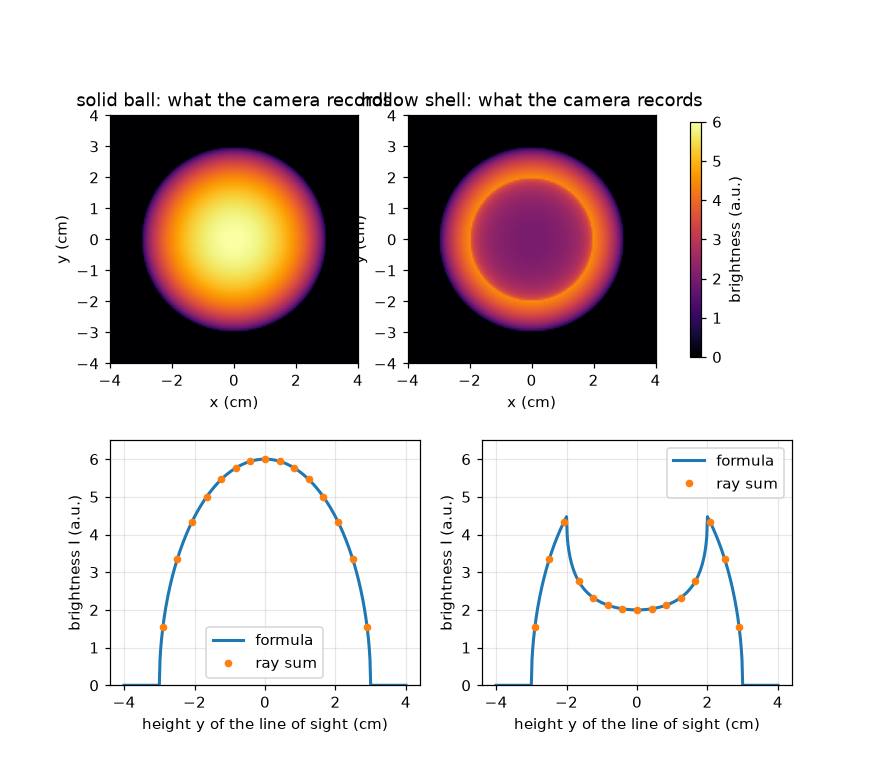
\includegraphics[width=0.85\linewidth]{figures/s01_ball_photos.png}\\\small Camera photos and brightness profiles of a solid glowing ball and a hollow shell (dots: brute-force ray sums).\end{center}

\subsection*{E. Worked example}
A solid ball of radius R = 3 cm has emission eps0 = 2 a.u. per cm. What does the camera record on a line of sight at y = 1.8 cm?
\begin{enumerate}[nosep]
\item Square the numbers: R\textasciicircum{}2 = 9 and y\textasciicircum{}2 = 3.24.
\item R\textasciicircum{}2 - y\textasciicircum{}2 = 5.76 and its square root is 2.4 cm.
\item The chord is 2 * 2.4 = 4.8 cm.
\item Brightness = eps0 * chord = 2 a.u. per cm * 4.8 cm = 9.6 a.u.
\item Sanity check: the centre line would give 2 * 3 * 2 = 12 a.u., larger than 9.6 as it must be, and the units (a.u. per cm times cm) give a.u.
\end{enumerate}
\textbf{Answer.} The chord is 4.8 cm and the pixel records 9.6 a.u.

\subsection*{F. Questions}
\begin{enumerate}[nosep]
\item \textbf{Conceptual.} Why is the middle of a solid glowing ball the brightest pixel, and why can a hollow shell be brighter at its edge than in the middle?
\item \textbf{Numerical.} A solid ball has R = 2.5 cm and eps0 = 1.2 a.u. per cm. Find the chord and the brightness at y = 1.5 cm, and at y = 0. Check the units.
\item \textbf{Graph and simulation interpretation.} In the profile of the hollow shell (R = 3 cm, r\_in = 2 cm), where is the brightest point and what value does it have? Why is the centre only 2 a.u.?
\item \textbf{Design and optimisation challenge.} Design: a glowing shell has outer radius 3 cm. Choose the inner radius so that the centre brightness is at most half of the brightest brightness. Is a hole of radius 1 cm enough? Justify with a calculation.
\end{enumerate}

\section{Session 2: From a radial recipe to a photo: the forward Abel transform}

\subsection*{A. Real-world problem}
A real flame does not glow equally everywhere: it may glow in a bright core, or in a hollow ring around a dark centre. We describe it by an emission profile eps(r): the light made per millimetre of path at distance r from the axis. If we know eps(r), what will the camera record? And since a camera has a limited number of pixels, how many pixels across the flame do we need before our model of the photo is accurate to 1 percent?

\subsection*{B. Concept and theory}
Take a line of sight at offset y from the axis. Walk along it a distance u from its closest point to the axis: there the distance from the axis is r = sqrt(y\textasciicircum{}2 + u\textasciicircum{}2). Adding the glow along the whole line (both directions) gives the brightness I(y); we keep only the region r \textless{} R, where the flame lives. This map from eps(r) to I(y) is the forward Abel transform. The integral can be written with u (no division by zero, so the trapezoid rule works). For a Gaussian eps = exp(-r\textasciicircum{}2/a\textasciicircum{}2) (a is its width) the answer is exactly a Gaussian again, I = sqrt(pi) a exp(-y\textasciicircum{}2/a\textasciicircum{}2). A camera works with pixels, so we cut the region into N rings of width dr = R/N and assume eps is constant in each ring. The line of sight at y\_i = i dr crosses ring j (for j \textgreater{}= i) along the length W\_ij; then I\_i is the sum over j of W\_ij eps\_j, which is a matrix times a vector. Lines of sight at y\_i never meet rings inside y\_i, so W is zero below its diagonal.

\begin{itemize}[nosep]
\item eps(r): emission at distance r from the axis (a.u. per mm)
\item I(y): brightness recorded at offset y (a.u.)
\item u: distance along the line of sight from its closest point to the axis (mm)
\item R: outer radius of the modelled region (4 mm) (mm)
\item a: width of the Gaussian flame (mm)
\item N, dr: number of rings and ring width R/N (no unit, mm)
\item W\_ij: path length of line of sight i inside ring j (mm)
\end{itemize}

\begin{equation*}
I(y)=2\int_0^{\sqrt{R^2-y^2}}\varepsilon\!\left(\sqrt{y^2+u^2}\right)\mathrm{d}u=2\int_y^{R}\frac{\varepsilon(r)\,r\,\mathrm{d}r}{\sqrt{r^2-y^2}}
\end{equation*}

\begin{equation*}
\varepsilon(r)=e^{-r^2/a^2}\ \Longrightarrow\ I(y)=\sqrt{\pi}\,a\,e^{-y^2/a^2}
\end{equation*}

\begin{equation*}
W_{ij}=2\left(\sqrt{r_{j+1}^2-y_i^2}-\sqrt{\max(r_j^2-y_i^2,0)}\right),\qquad I_i=\sum_{j\ge i}W_{ij}\,\varepsilon_j
\end{equation*}

\begin{center}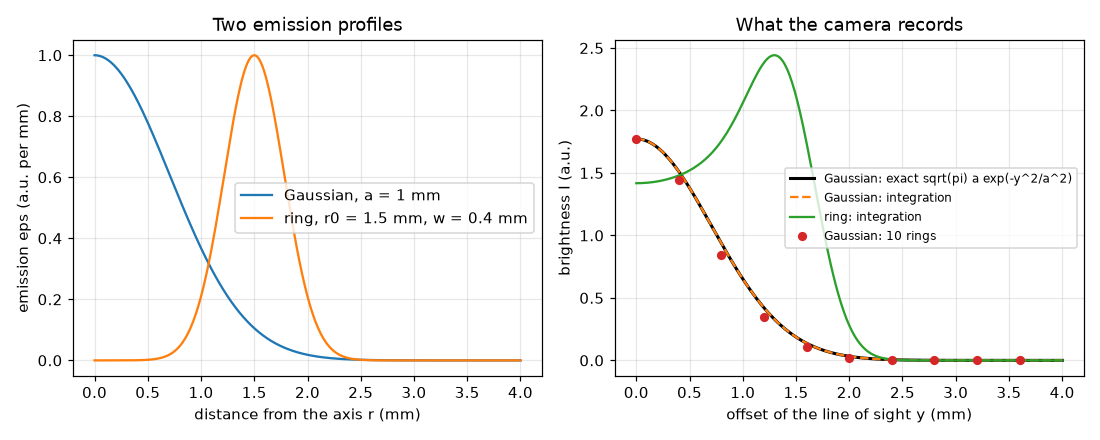
\includegraphics[width=0.85\linewidth]{figures/s02_forward_profiles.png}\\\small Left: Gaussian and ring emission profiles. Right: the photo profiles; red dots are a 10-ring model.\end{center}

\subsection*{E. Worked example}
For a Gaussian flame with a = 1 mm, what brightness does the camera record at y = 1 mm? Check it with numerical integration.
\begin{enumerate}[nosep]
\item Use I(y) = sqrt(pi) a exp(-y\textasciicircum{}2 / a\textasciicircum{}2) with a = 1 and y = 1.
\item The exponent is -1\textasciicircum{}2 / 1\textasciicircum{}2 = -1, and exp(-1) = 0.3679.
\item sqrt(pi) = 1.7725, so I = 1.7725 * 0.3679 = 0.652 a.u.
\item Numerical check: integrate 2 exp(-(1 + u\textasciicircum{}2)) over u from 0 to 3 with the trapezoid rule; the code \texttt{abel\_forward} gives 0.652.
\item Sanity check: the peak (y = 0) is sqrt(pi) = 1.77 a.u., so 0.652 is smaller, as it must be at a line of sight away from the axis.
\end{enumerate}
\textbf{Answer.} I(1 mm) = sqrt(pi)/e = 0.652 a.u.; the numerical integral agrees.

\subsection*{F. Questions}
\begin{enumerate}[nosep]
\item \textbf{Conceptual.} Why must the ring matrix W be zero below its diagonal? What does that mean for solving the inverse problem?
\item \textbf{Numerical.} A Gaussian flame has width a = 0.5 mm. What is the brightness at y = 0 and at y = 0.5 mm? Give the units and a sanity check.
\item \textbf{Graph and simulation interpretation.} On the plot of ring-model error against N, how does the error change from N = 10 to N = 40 for a = 1 mm? Read the numbers and say what happens when the flame is narrower.
\item \textbf{Design and optimisation challenge.} Design: a camera images a region 8 mm wide in total (R = 4 mm on each side of the axis). The flame is a Gaussian with a = 0.7 mm and you want the ring model accurate to 1 percent of the peak. How many pixels across the whole image (both sides) and what pixel size do you need? What happens if the flame is half as wide?
\end{enumerate}

\section{Session 3: Back from the photo: onion peeling, noise and smoothing}

\subsection*{A. Real-world problem}
You have a photo of a flame and you want the glow of its inside, for example the radial profile of soot or temperature, not the sum along each line of sight. If the flame is round about its axis one photo is enough. But every real photo has a little noise, and the inversion makes it worse. How much worse, where, and what can you do about it without cheating? (This is a teaching model; real combustion diagnostics need calibration and many more checks.)

\subsection*{B. Concept and theory}
Session 2 gave I = W eps, with W upper triangular. Onion peeling solves it from the outside in: the outermost ring from the outermost pixel, then each inner ring after subtracting what the outer rings already explain. With perfect data this is exact for the ring model. With noise, errors accumulate towards the axis. Because the inversion is linear, eps = Winv I, so noise of standard deviation sigma on each pixel gives noise of sigma times the length of row i of Winv on ring i; call that length the noise gain. To tame the noise we ask for a smooth answer: minimise the misfit \textbar{}W eps - I\textbar{}\textasciicircum{}2 plus lam times the roughness \textbar{}D eps\textbar{}\textasciicircum{}2, where D takes second differences (zero for a straight-line profile). Large lam gives a smooth but biased profile, lam = 0 gives noisy onion peeling. The total error combines the bias (the average error) and the noise (the scatter): total\textasciicircum{}2 = bias\textasciicircum{}2 + noise\textasciicircum{}2. To avoid an inverse crime (testing with data made by the same approximation), the test photos are made by a fine numerical integral.

\begin{itemize}[nosep]
\item eps\_i: emission of ring i (a.u. per mm)
\item I\_i: brightness at offset y\_i (a.u.)
\item sigma: standard deviation of the photo noise (fraction of the peak brightness) (a.u.)
\item gain\_i: noise gain: noise in ring i divided by sigma (per mm)
\item lam: smoothing strength (scaled so it has no unit) (no unit)
\item bias, noise, total: RMS errors as a fraction of the peak emission (no unit)
\end{itemize}

\begin{equation*}
I_i=\sum_{j\ge i}W_{ij}\varepsilon_j\ \Longrightarrow\ \varepsilon_i=\frac{I_i-\sum_{j>i}W_{ij}\varepsilon_j}{W_{ii}}
\end{equation*}

\begin{equation*}
\mathrm{gain}_i=\Big(\sum_k (W^{-1})_{ik}^2\Big)^{1/2},\qquad \sigma_{\varepsilon,i}=\sigma\cdot\mathrm{gain}_i
\end{equation*}

\begin{equation*}
\hat{\varepsilon}=\arg\min_{\varepsilon}\ \|W\varepsilon-I\|^2+\lambda s\,\|D\varepsilon\|^2=(W^{\mathsf T}W+\lambda s D^{\mathsf T}D)^{-1}W^{\mathsf T}I
\end{equation*}

\begin{equation*}
\mathrm{total}^2=\mathrm{bias}^2+\mathrm{noise}^2
\end{equation*}

\begin{center}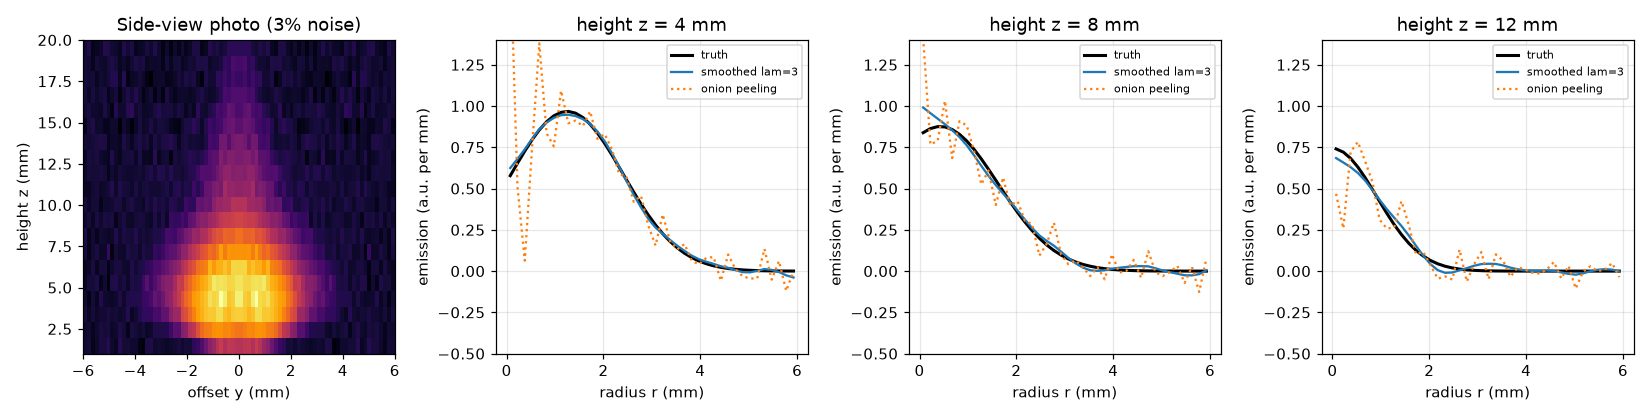
\includegraphics[width=0.85\linewidth]{figures/s03_candle_rows.png}\\\small Synthetic candle photo with 3 percent noise and the recovered radial emission at three heights.\end{center}

\subsection*{E. Worked example}
Three rings of width 1 mm (R = 3 mm) give measured brightness I = (12, 9.121, 4.472) a.u. at y = 0, 1 and 2 mm. Recover the emission of each ring by onion peeling.
\begin{enumerate}[nosep]
\item The ring matrix (Session 2 formula) has rows (2, 2, 2), (0, 3.464, 2.192) and (0, 0, 4.472).
\item Outermost ring first: eps\_2 = 4.472 / 4.472 = 1.
\item Next ring: eps\_1 = (9.121 - 2.192 * 1) / 3.464 = 6.929 / 3.464 = 2.
\item Innermost ring: eps\_0 = (12 - 2 * 2 - 2 * 1) / 2 = 6 / 2 = 3.
\item Check by the forward model: 2*3 + 2*2 + 2*1 = 12, 3.464*2 + 2.192*1 = 9.120 and 4.472*1 = 4.472, which reproduce the measured values.
\end{enumerate}
\textbf{Answer.} The emission is (3, 2, 1) a.u. per mm, from the axis outwards.

\subsection*{F. Questions}
\begin{enumerate}[nosep]
\item \textbf{Conceptual.} Why does the noise in the recovered emission grow towards the axis, and why does smoothing help but not for free?
\item \textbf{Numerical.} For N = 40 rings the noise gain of the axis ring is 5.9 per mm. The photo noise is sigma = 0.02 a.u. What is the noise in the emission of the axis ring? Compare with a Gaussian flame whose peak emission is 1 a.u. per mm.
\item \textbf{Graph and simulation interpretation.} On the trade-off graph of the Gaussian flame at 1 percent noise, how do the bias, noise and total change as lam goes from 0.00001 to 30? Where is the minimum of the total?
\item \textbf{Design and optimisation challenge.} Design: a ring-shaped flame (r0 = 1.5 mm, w = 0.4 mm) is photographed with 1 percent noise and 40 rings. Choose between lam = 0.01, 0.1 and 10 and give the total error of each (use \texttt{bias\_noise\_exact}). What risk does the largest lam bring for a hollow flame?
\end{enumerate}

\section{Real-world mini-project}
\textbf{Recover the inside of a candle-like flame from a synthetic photo.} A lab gives you a synthetic side-view photograph of a candle-like flame with 3 percent noise (\texttt{candle\_photo(N=40, frac=0.03)} in Session 3). The flame is hollow near its base and fills in higher up. Recover the radial emission at three heights (z = 4, 8 and 12 mm) with \texttt{invert\_row}, trying the smoothing strengths in \texttt{LAM\_GRID}, and choose the one with the smallest worst-row error. Because this is a synthetic photo, the true emission \texttt{candle\_emission} is known, so you can score each choice.

\section{The path ahead}
\begin{enumerate}[nosep]
\item \textbf{Session 4: Choose the smoothing from the photo alone.} A function that selects lam from a single noisy photo, replacing the grid search that peeks at the true profile.
\item \textbf{Session 5: Find the flame axis.} An axis finder with sub-pixel accuracy, used before the inversion.
\item \textbf{Session 6: Use both sides and neighbouring rows.} A whole-image inversion of all 20 rows with less noise than row-by-row inversion.
\item \textbf{Session 7: Keep the hollow base hollow.} An inversion that keeps the dark core of the candle base without negative values.
\item \textbf{Session 8: Render it in 3D and animate.} A looping 3D cut-away animation of the recovered flame.
\end{enumerate}

\section{Answers and hints}

\subsection*{Session 1}
\begin{enumerate}[nosep]
\item \textbf{Conceptual.} Hint: Compare the path lengths through glowing material for a line through the middle and a line near the edge of the hole. Solution: The pixel adds up light along the path, so a longer path through glowing material gives a brighter pixel. In a solid ball the line through the middle is the longest. In a shell the middle line spends most of its length in the empty hole, so only the short walls count; a line that just grazes the hole travels a long way inside the wall, so the brightest line is the one that touches the inner radius.
\item \textbf{Numerical.} Hint: Use chord = 2 sqrt(R\textasciicircum{}2 - y\textasciicircum{}2): at y = 1.5, R\textasciicircum{}2 - y\textasciicircum{}2 = 6.25 - 2.25 = 4. Solution: At y = 1.5 cm: chord = 2 * sqrt(4) = 4 cm and I = 1.2 * 4 = 4.8 a.u. At y = 0: chord = 2R = 5 cm and I = 1.2 * 5 = 6.0 a.u. Units: (a.u. per cm) times cm = a.u. Sanity: the off-centre line is shorter so it is dimmer.
\item \textbf{Graph and simulation interpretation.} Hint: The brightest line touches the inner circle: y = r\_in. Evaluate 2 sqrt(R\textasciicircum{}2 - r\_in\textasciicircum{}2). Solution: The brightest point is at y = 2 cm with I = 2 sqrt(9 - 4) = 2 sqrt(5) = 4.47 a.u. The centre line has chord 6 cm through the outer ball minus 4 cm through the hole, so 2 cm and I = 2 a.u. The profile therefore has a dip in the middle and two bright shoulders, called limb brightening.
\item \textbf{Design and optimisation challenge.} Hint: The ratio I(0) / I\_max = sqrt((R - r\_in) / (R + r\_in)). Set it to 1/2. Solution: I(0) / I\_max = sqrt((R - r\_in) / (R + r\_in)) \textless{}= 1/2 means (R - r\_in) / (R + r\_in) \textless{}= 1/4, so r\_in \textgreater{}= 0.6 R = 1.8 cm. A hole of 1 cm is not enough: the ratio is sqrt(2/4) = 0.71. With r\_in = 2 cm the ratio is sqrt(1/5) = 0.45, which works. Trade-off: a bigger hole gives a stronger dark centre but a thinner glowing wall, so the whole image is dimmer.
\end{enumerate}

\subsection*{Session 2}
\begin{enumerate}[nosep]
\item \textbf{Conceptual.} Hint: Which rings can the line of sight at y\_i cross? Solution: A line of sight at offset y\_i stays at a distance of at least y\_i from the axis, so it can only cross rings whose outer edge is beyond y\_i, that is rings j \textgreater{}= i. Rings inside y\_i give W\_ij = 0. Because W is triangular, the outermost line of sight meets only the outermost ring, the next one meets two rings, and so on: the inverse can be solved ring by ring from the outside inwards (onion peeling, Session 3).
\item \textbf{Numerical.} Hint: I(y) = sqrt(pi) a exp(-y\textasciicircum{}2/a\textasciicircum{}2). Solution: At y = 0: I = 1.7725 * 0.5 = 0.886 a.u. At y = 0.5 mm: I = 0.886 * exp(-1) = 0.326 a.u. Units: eps in a.u. per mm times mm gives a.u. Sanity: a narrower flame has a smaller total (0.886 against 1.77 for a = 1 mm) and the value falls to 1/e = 37 percent of the peak at y = a.
\item \textbf{Graph and simulation interpretation.} Hint: The checkpoint prints the exact values; the curves for a = 0.5 and a = 0.7 are above the one for a = 1. Solution: For a = 1 mm the error is 5.4 percent at N = 10, 2.0 percent at N = 20 and 0.7 percent at N = 40: it falls roughly like dr to the power 1.4 (each halving of the pixel size divides the error by about 2.7). Narrower flames have larger errors at the same N because the profile changes faster across a ring; the a = 0.5 mm curve needs about twice as many rings to reach the same error.
\item \textbf{Design and optimisation challenge.} Hint: Use \texttt{smallest\_rings(0.7)}; pixels across = 2N; pixel size = R / N. Solution: smallest\_rings(0.7) = 47 rings, so the 8 mm wide image needs 2 * 47 = 94 pixels across, with pixel size 4 / 47 = 0.085 mm. For a = 0.5 mm the answer is 65 rings (pixel 0.062 mm); for a = 1 mm it is 33 rings (pixel 0.121 mm). In all three cases the pixel size is about 0.12 times the width a, that is about 8 pixels across one Gaussian width a. Trade-off: finer pixels need a closer or better camera and gather less light per pixel, which raises the noise (Session 3).
\end{enumerate}

\subsection*{Session 3}
\begin{enumerate}[nosep]
\item \textbf{Conceptual.} Hint: Think about how many pixels' errors are added up in the innermost ring. Solution: Each inner ring is found by subtracting the contribution of all outer rings from the pixel, so the errors of all the outer solutions pile up, and then they are divided by W\_ii = 2 dr sqrt(2i + 1), which is smallest for the axis ring (i = 0). The noise gain is about 5.9 per mm at the axis and 0.56 per mm at the edge (N = 40). Smoothing averages neighbouring rings, which cancels random noise, but it also averages real structure, so sharp features (a peak, a hole) are lowered and blurred: this is the bias. The total error is smallest when the two are balanced.
\item \textbf{Numerical.} Hint: noise = sigma * gain; then divide by the peak. Solution: noise = 0.02 a.u. * 5.9 per mm = 0.12 a.u. per mm. Relative to the peak of 1 a.u. per mm that is 12 percent, six times the 2 percent noise of the photo. The outer ring has gain 0.56 per mm and noise 0.011 a.u. per mm (1 percent). Units: a.u. times per mm is a.u. per mm, the unit of the emission.
\item \textbf{Graph and simulation interpretation.} Hint: Move the log10 lam slider in the app or read the third panel of the figure. Solution: The bias is flat at about 0.4 percent for small lam and rises to about 1.9 percent at lam = 30. The noise falls steadily from about 2.7 percent to about 0.4 percent. The total is about 2.7 percent for tiny lam, falls to a minimum of about 1.1 percent near lam = 0.3 (log10 lam = -0.5), then rises again as the bias takes over. The best choice is the one at the valley, not the largest lam.
\item \textbf{Design and optimisation challenge.} Hint: Print \texttt{bias\_noise\_exact(lambda q: ring\_eps(q, 1.5, 0.4), 40, lam, 0.01)} for the three values. Solution: The total errors are about 2.7 percent for lam = 0.01 (noise dominates), 2.0 percent for lam = 0.1 (best) and 7.7 percent for lam = 10 (bias dominates). Choose lam = 0.1. With lam = 10 or more, smoothing lowers the ring peak and fills or even drives negative the dark hole on the axis, so the flame would be misread as less hollow and with negative emission, which is unphysical. Trade-off: a ring flame needs less smoothing than a Gaussian flame because it has sharper structure.
\end{enumerate}

\section{How to join}
Read \texttt{CONTRIBUTING.md} in the repository, then pick an issue labelled \texttt{good first issue}. Repository: \url{https://github.com/KrunalPanchal1995/openabel}

\end{document}
